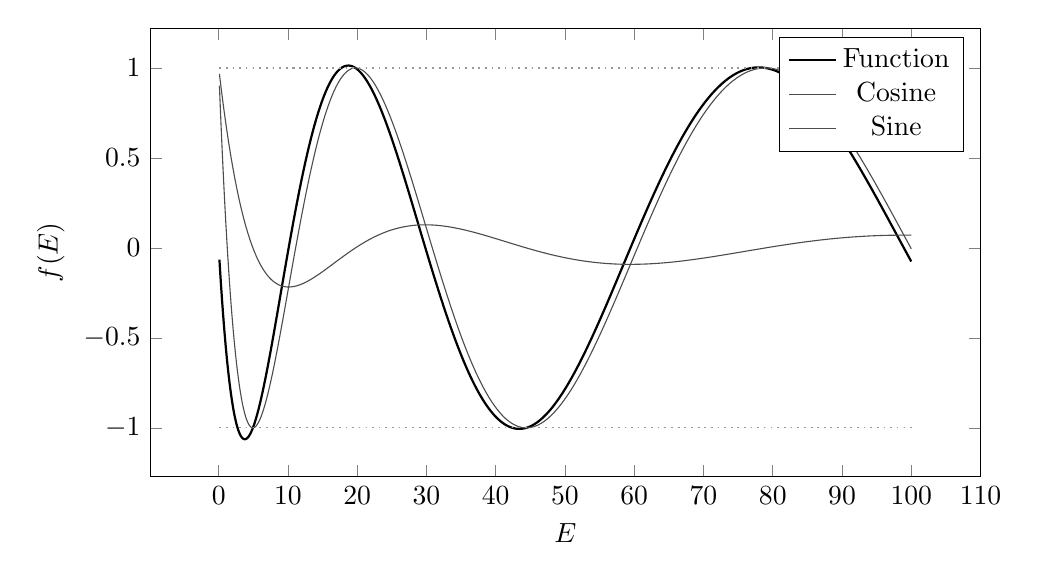
\begin{tikzpicture}
    \begin{axis}[
            width=\linewidth,
            height=.6\linewidth,
            domain=.1:100,
            samples=1000,
            xlabel=$E$,
            ylabel=$f(E)$,
        ]
        \addplot[black, thick] {-sin(deg(sqrt(2*x))) / sqrt(2*x) + cos(deg(sqrt(2*x)))};
        \addplot[black!70] {cos(deg(sqrt(2*x)))};
        \addplot[black!70] {sin(deg(sqrt(2*x))) / sqrt(2*x)};
        \addplot[black!40, dotted] {1};
        \addplot[black!40, dotted] {-1};
        \addlegendentry{Function}
        \addlegendentry{Cosine}
        \addlegendentry{Sine}
    \end{axis}
\end{tikzpicture}
